\section{Thống kê mô tả}
\subsection{Thống kê mô tả cho các biến định lượng}
Ta tiến hành tính thống kê mô tả cho các biến định lượng (\textbf{Code[33]$\rightarrow$[36]}).
\begin{figure}[H]
    \centering
    
\includegraphics[width=0.8\linewidth]{
    IMAGES/4.png}
    \caption{Kết quả khi kiểm tính thống kê mô tả cho các biến định lượng}
    \label{fig9}
\end{figure}
\textbf{\textit{Nhận xét}}: Hình~\ref{fig9} Dựa vào các số liệu thống kê, ta có thể rút ra một số nhận xét như sau:

Ta thấy biến order\_total có giá trị trung bình là 39,209.67, cao hơn nhiều so với giá trị trung vị là 11,293.96. Điều này chứng tỏ rằng phân phối của dữ liệu bị lệch phải, do một số đơn hàng có giá trị rất lớn kéo trung bình lên cao. Ngoài ra, giá trị lớn nhất của biến này là 5,688,269.6, trong khi giá trị nhỏ nhất chỉ là 639.29. Sự chênh lệch lớn giữa các đơn hàng thể hiện mức độ không đồng đều trong dữ liệu.

Ta thấy biến delivery\_charges có giá trị trung bình là 76.658 và giá trị trung vị là 76.31, phản ánh phân phối dữ liệu khá đối xứng. Khoảng dao động của phí giao hàng cũng không lớn, với giá trị nhỏ nhất là 46.35 và giá trị lớn nhất là 114.04. Điều này cho thấy sự ổn định của phí giao hàng trong các đơn hàng.

Ta thấy biến order\_price có giá trị trung bình là 25,522.22, cao hơn giá trị trung vị là 12,807.50. Sự chênh lệch này phản ánh sự xuất hiện của một số đơn hàng có giá trị rất cao, dẫn đến trung bình bị kéo lên. Giá trị lớn nhất là 947,691, trong khi giá trị nhỏ nhất là 585. Sự khác biệt lớn này cho thấy sự đa dạng đáng kể trong giá trị các đơn hàng.

Ta thấy biến distance\_to\_nearest\_warehouse có giá trị trung bình là 2.20 km và giá trị trung vị là 1.03 km. Phần lớn khách hàng có khoảng cách gần với kho, nhưng giá trị lớn nhất lên tới 94.97 km lại chỉ ra rằng một số khách hàng ở rất xa. Đây có thể là các trường hợp ngoại lệ hoặc thuộc khu vực đặc biệt.

Tóm lại, ta thấy các biến order\_total và order\_price có phân phối không đồng đều do ảnh hưởng của các giá trị ngoại lai lớn, trong khi các biến delivery\_charges và distance\_to\_nearest\_w-arehouse lại có sự ổn định hơn. Ta cần kiểm tra thêm các giá trị ngoại lai và phân tích mối tương quan giữa các biến để đưa ra các kết luận chính xác và ý nghĩa hơn.
\subsection{Thống kê số lượng cho các biến phân loại}
Ta tiến hành lập bảng thống kê số lượng cho mỗi phân loại của biến (\textbf{Code[39]}).
\begin{figure}[H]
    \centering
    
\includegraphics[width=0.8\linewidth]{IMAGES/5.png}
    \caption{Kết quả khi lập bảng thống kê số lượng mỗi phân loại của biến season}
    \label{fig10}
\end{figure}
\textbf{\textit{Nhận xét}}: Kết quả hình~\ref{fig10} cho ta thấy rằng mùa thu (Autumn) là mùa xuất hiện nhiều nhất trong dữ liệu, trong khi mùa hè (Summer) lại là mùa ít xuất hiện nhất. Dựa trên điều này, ta có thể dự đoán rằng lượng đặt hàng vào mùa thu sẽ cao đáng kể so với các mùa còn lại. Điều này có thể chỉ ra rằng vào mùa thu, số lượng đơn hàng thường tăng lên, không phải do xu hướng mua sắm nhiều hơn mà có thể là do các chính sách ưu đãi đặc biệt được áp dụng trong mùa này. Như vậy, ta cần nghiên cứu thêm các yếu tố khác như chương trình khuyến mãi hoặc nhu cầu thị trường để hiểu rõ hơn về sự gia tăng đơn hàng trong mùa thu.

Ta tiếp tục lập bảng thống kê số lượng cho mỗi phân loại của biến is\_expedited\_delivery (\textbf{Code[40]}).

\begin{figure}[H]
    \centering
    \captionsetup{justification=centering, margin = 2cm}
    
\includegraphics[width=0.5\linewidth]{IMAGES/6.png}
    \caption{Kết quả khi lập bảng thống kê số lượng mỗi phân loại của biến is\_expedited\_delivery
table (new\_data\$is\_expedited\_delivery)}
    \label{fig11}
\end{figure}
\textbf{\textit{Nhận xét}}: Hình~\ref{fig11} Ta có thể đánh giá được lượng khách hàng chọn giao hàng nhanh ít lượng khách hàng không chọn nhưng không đáng kể. Qua đó cho thấy khách hàng không quan tâm tới thời gian giao hàng hoặc chọn giao chậm để tiết kiệm chi phí.

Ta tiếp tục lập bảng thống kê số lượng cho mỗi phân loại của biến nearest\_warehouse (\textbf{Code[38]}).
\begin{figure}[H]
    \centering
    
\includegraphics[scale =1.25]{
    IMAGES/7.png}
    \caption{Kết quả khi lập bảng thống kê số lượng mỗi phân loại của biến nearest\_warehouse}
    \label{fig12}
\end{figure}
\textbf{\textit{Nhận xét}}: Hình~\ref{fig12} Bảng thống kê cho thấy, ta có thể nhận thấy rằng kho Thomson giữ 39.4\% hàng hóa, kho Nicholson 36.8\%, và kho Bakers 23.8\%. Điều này chỉ ra rằng kho Thomson có vị trí địa lý thuận lợi, giúp ta nhận định rằng kho này có thể đáp ứng nhu cầu khách hàng tốt hơn các kho còn lại, từ đó hỗ trợ ta xây dựng chiến lược phát triển hiệu quả hơn.

Ta lập bảng thống kê số lượng cho mỗi phân loại của biến is\_happy\_customer (\textbf{Code[41]}).
\begin{figure}[H]
    \centering
    
\includegraphics[scale =1.5]{
    IMAGES/8.png}
    \caption{Kết quả khi lập bảng thống kê sự hài lòng của khách hàng is\_happy\_customer }
    \label{fig13}
\end{figure}
\textbf{\textit{Nhận xét}}: Hình~\ref{fig13} 
Trong tổng số 500 đơn đặt hàng, ta thấy có 359 đơn hài lòng với dịch vụ, chiếm 71.8\%, xấp xỉ 3/4 số khách hàng. Điều này cho thấy phần lớn khách hàng cảm thấy hài lòng với dịch vụ hiện tại. Tuy nhiên, ta cũng nhận thấy vẫn còn 28.2\% khách hàng không hài lòng, một tỷ lệ không nhỏ. Sự không hài lòng này có thể phản ánh những vấn đề chưa được đáp ứng đầy đủ trong dịch vụ khách hàng, có thể là về thời gian giao hàng, chất lượng sản phẩm hay trải nghiệm mua sắm. Do đó, ta cần thực hiện các biện pháp để cải thiện chất lượng phục vụ, như nâng cao khả năng giao hàng nhanh chóng, cải thiện dịch vụ chăm sóc khách hàng, và đảm bảo chất lượng sản phẩm ổn định để tăng sự hài lòng và giảm tỷ lệ khách hàng không hài lòng.
\subsection{Mô tả dữ liệu bằng đồ thị}
\subsubsection{Đồ thị Histogram}
Ta tiến hành vẽ đồ thị Histogram thể hiện phân phối của order\_total, delivery\_charges, order\_price, distance\_to\_nearest\_warehouse và coupon\_discount (\textbf{Code[43]$\rightarrow$[48]}).
\begin{figure}[H]
    \centering
    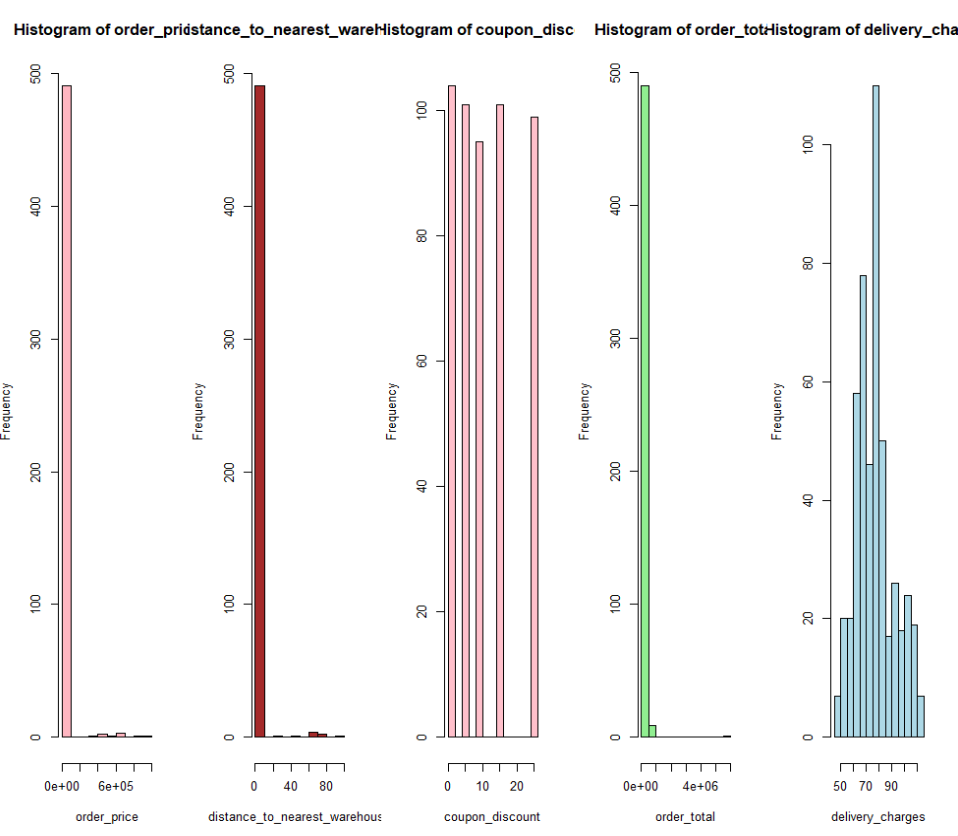
\includegraphics[scale=0.55]{IMAGES/51.png}
    \caption{Kết quả khi vẽ đồ thị Histogram thể hiện phân phối của các biến.}
    \label{fig14}
\end{figure}

\textbf{\textit{Nhận xét}}: Hình~\ref{fig14} Từ các biểu đồ trên, ta thấy rằng ba trên năm biểu đồ có phân phối lệch phải, với một cột cao ở phía bên trái. Điều này chủ yếu do sự hiện diện của các điểm ngoại lai, khiến việc nhận dạng phân phối biến trở nên khó khăn. Để xử lý vấn đề này, ta sẽ sử dụng lý thuyết phân vị và chuyển các giá trị nằm ngoài khoảng giới hạn (tính theo công thức [Q1 - 1.5 * IQR] đến [Q3 + 1.5 * IQR]) thành NA và loại bỏ các điểm ngoại lai này (nếu giá trị ngoại lai không đáng kể) bằng cách sử dụng hàm \textbf{na.omit}.(\textbf{Code[50]$\rightarrow$[70]}).
\begin{figure}[H]
    \centering
    \captionsetup{justification=centering, margin = 2cm}
    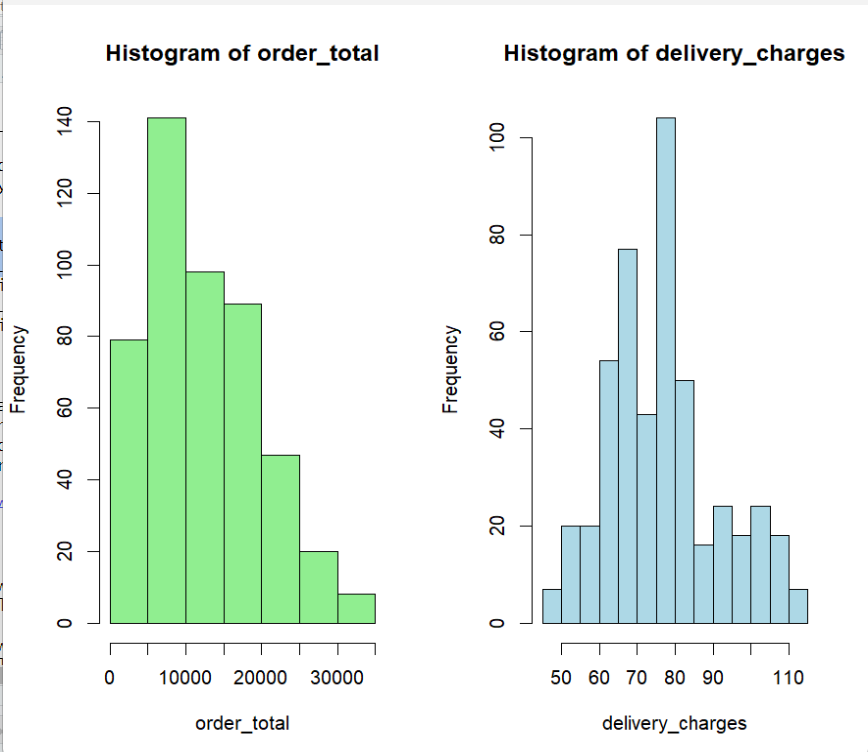
\includegraphics[scale =0.35]{IMAGES/16.png}
    \caption{Kết quả khi vẽ đồ thị Histogram sau khi xử lí thể hiện phân phối của order\_total và delivery\_charges.}
    \label{fig15}
\end{figure}
\textbf{\textit{Nhận xét}}: \\
Hình~\ref{fig15} Ta thấy được:
\begin{itemize}
    \setlength{\itemsep}{0pt}
    
   \item Ta thấy histogram của biến order\_total cho thấy phân phối lệch trái, với phần lớn giá trị trong khoảng 0-15.000 và tần suất cao nhất ở khoảng 0-10.000. Từ 10.000 trở đi, tần suất giảm dần, cho thấy các đơn hàng giá trị cao ít phổ biến. Các đơn hàng trên 30.000 rất hiếm, gợi ý rằng ta thấy đa số khách hàng chỉ đặt các đơn hàng nhỏ.

\item Ta thấy histogram của biến delivery\_charges cho thấy phân phối gần như đối xứng, với phần lớn giá trị trong khoảng 70-90 và tần suất cao nhất ở khoảng 80. Phân phối có dạng chuông, cho thấy mức phí giao hàng thường dao động quanh giá trị trung bình. Phí giao hàng thấp dưới 60 hoặc cao trên 100 rất hiếm, phản ánh chi phí giao hàng ổn định trong một phạm vi nhất định, điều này cho thấy ta nhận thấy mức phí giao hàng khá đồng đều.
\end{itemize}




\begin{figure}[H]
    \centering
    \captionsetup{justification=centering, margin = 2cm}
    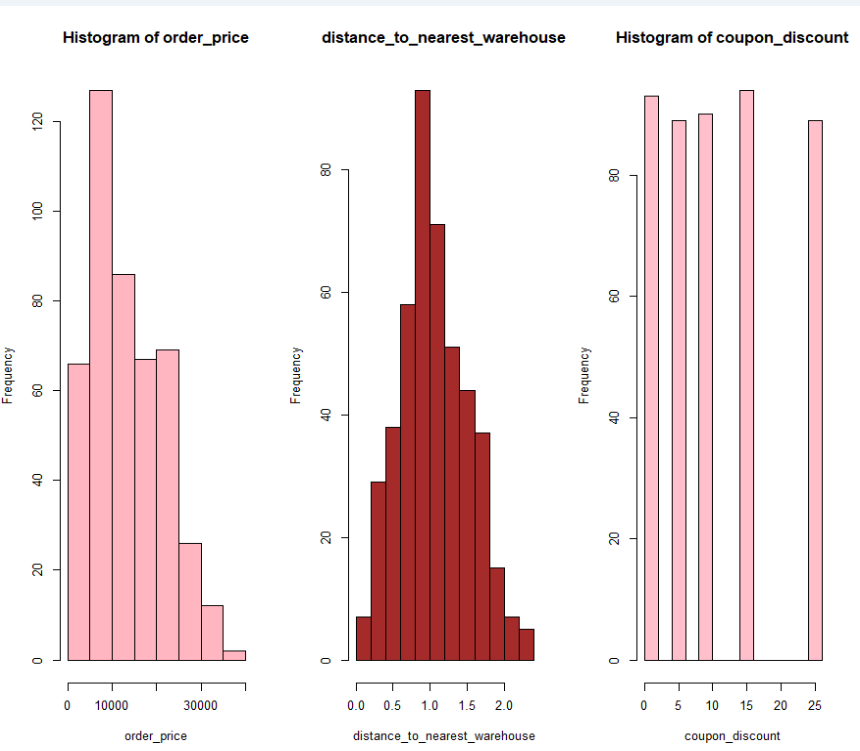
\includegraphics[scale =0.3]{IMAGES/17.png}
    \caption{Kết quả khi vẽ đồ thị Histogram sau khi xử lí thể hiện phân phối của order\_price, distance\_to\_nearest\_warehouse và coupon\_discount.}
    \label{fig16}
\end{figure}
\textbf{\textit{Nhận xét}}:\\
Hình~\ref{fig16} Ta thấy được:
\begin{itemize}
   \item Ta thấy histogram của biến order\_price cho thấy phân phối lệch phải, với phần lớn giá trị tập trung ở khoảng 0-10.000 và tần suất cao nhất đạt hơn 120. Sau mức 10.000, tần suất giảm rõ rệt, cho thấy các đơn hàng giá trị cao ít phổ biến. Điều này cho thấy hầu hết đơn hàng có giá trị nhỏ, và các đơn hàng giá trị lớn rất hiếm.

\item Ta thấy histogram của biến distance\_to\_nearest\_warehouse có dạng hình chuông, vẫn còn xu hướng lệch phải, phản ánh phân phối chuẩn. Khoảng cách đến kho gần nhất tập trung chủ yếu từ 0.5-1.5 (đơn vị không rõ), với tần suất cao nhất tại khoảng 1.0. Điều này cho thấy phần lớn khách hàng ở khoảng cách trung bình so với kho, và khoảng cách cực gần hoặc cực xa rất ít xảy ra.

\item Ta thấy histogram của biến coupon\_discount cho thấy dữ liệu phân bố dạng rời rạc, với các giá trị cụ thể (5, 10, 15, 20, 25) và tần suất tương đối đồng đều ở từng mức. Điều này có thể do các mức giảm giá cố định được thiết lập sẵn, phản ánh chính sách ưu đãi theo từng nấc cụ thể của doanh nghiệp.

\end{itemize}
\textbf{\textit{Nhận xét}}: Nhìn chung, ta thấy việc loại bỏ các điểm ngoại lai có thể giúp làm sạch dữ liệu và giảm ảnh hưởng của giá trị cực đoan. Tuy nhiên, dựa trên histogram hiện tại, dù các điểm ngoại lai đã được loại bỏ, ta vẫn thấy phân phối chưa đạt tính đối xứng gần như phân phối chuẩn và vẫn còn xu hướng lệch phải. Điều này cho thấy dữ liệu vẫn tồn tại sự thiên lệch và có thể cần thêm bước xử lý trước khi áp dụng các phương pháp thống kê yêu cầu giả định phân phối chuẩn.
\subsubsection{Đồ thị Boxplot}

Vẽ biểu đồ Boxplot thể hiện phân phối của order\_total theo season (\textbf{Code[72]})
\begin{figure}[H]
    \centering
    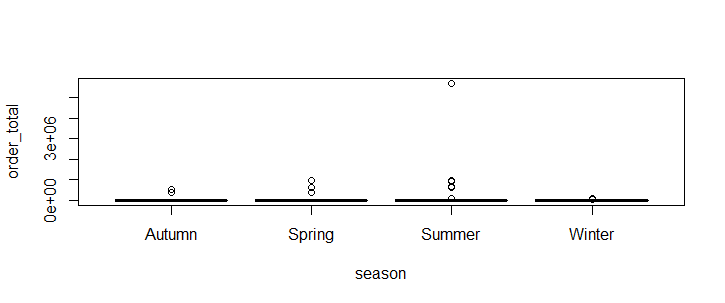
\includegraphics[width=0.8\linewidth]{IMAGES/10.png}
    \caption{Kết quả khi vẽ Boxplot thể hiện phân phối của order\_total theo season.}
    \label{fig17}
\end{figure}
\textbf{\textit{Nhận xét}}: Hình~\ref{fig17} Đồ thị cho thấy có nhiều điểm ngoại lai xa khiến ta không thể so sánh được phân phối của order\_total theo season. Vì thế ta sẽ thực hiện đề xuất phương pháp phù hợp để xử lý các ngoại lai này.
\\
Ta thực hiện tạo hàm tìm các ngoại lai và chuyển ngoại lai thành NA (\textbf{Code[74]$\rightarrow$[81]}) 
\begin{figure}[H]
    \centering
    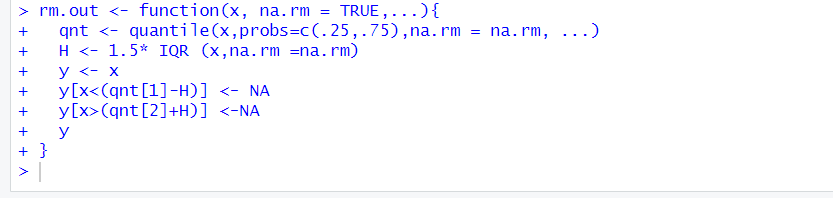
\includegraphics[scale =0.5]{IMAGES/40.png}
    \caption{(Tiến hành thực hiện xử lí).}
    \label{fig:hinh19}
\end{figure}
Sau đó, ta thực hiện sử dụng hàm vừa tạo và thực hiện trên các bộ dữ liệu được phân theo season (\textbf{Code[82]$\rightarrow$[96]}).
\begin{figure}[H]
    \centering
    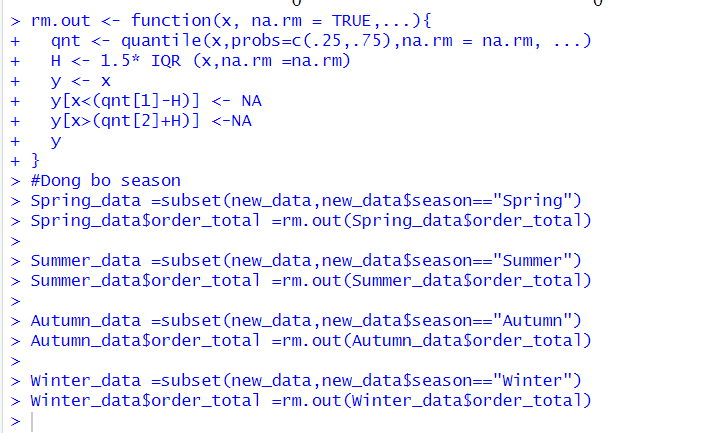
\includegraphics[scale =0.4]{IMAGES/53.png}
    \caption{Kết quả khi kiểm tra các dữ liệu NA (là các ngoại lai được tìm thấy).}
    \label{fig:hinh20}
\end{figure}
Sau đó ta ghép các bộ dữ liệu sau khi tìm ngoại lại và thực hiện kiểm tra các dữ liệu NA (là các ngoại lai được tìm thấy) (\textbf{Code[95]$\rightarrow$[98]}).
Kết quả:
\begin{figure}[H]
    \centering
    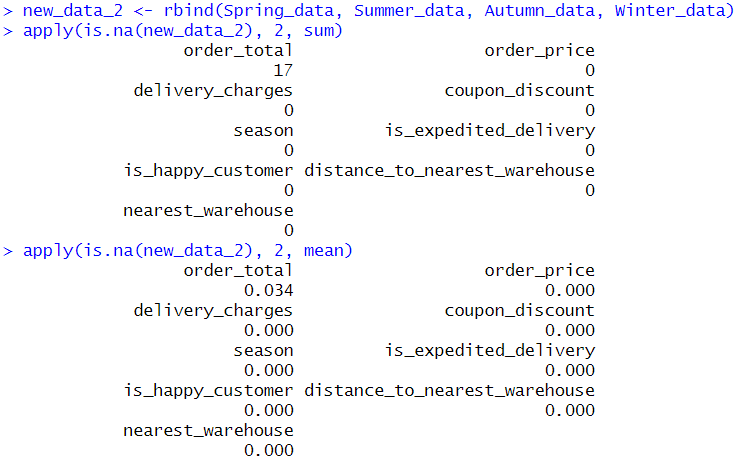
\includegraphics[scale = 0.5]{IMAGES/11.png}
    \caption{Kết quả khi kiểm tra các dữ liệu NA (là các ngoại lai được tìm thấy).}
    \label{fig20}
\end{figure}
\textbf{\textit{Nhận xét}}: Hình~\ref{fig20} Ta tìm thấy 17 quan sát là ngoại lai (chiếm tỷ lệ 3.4\% so với toàn bộ quan sát). Vì lượng dữ liệu ngoại lai nhỏ nên sai số sẽ không đáng kể. Vì vậy, ta sẽ chọn phương pháp xoá các các giá trị ngoại lai này và vẽ lại đồ thị (\textbf{Code[100]$\rightarrow$[101]}).
\begin{figure}[H]
    \centering
    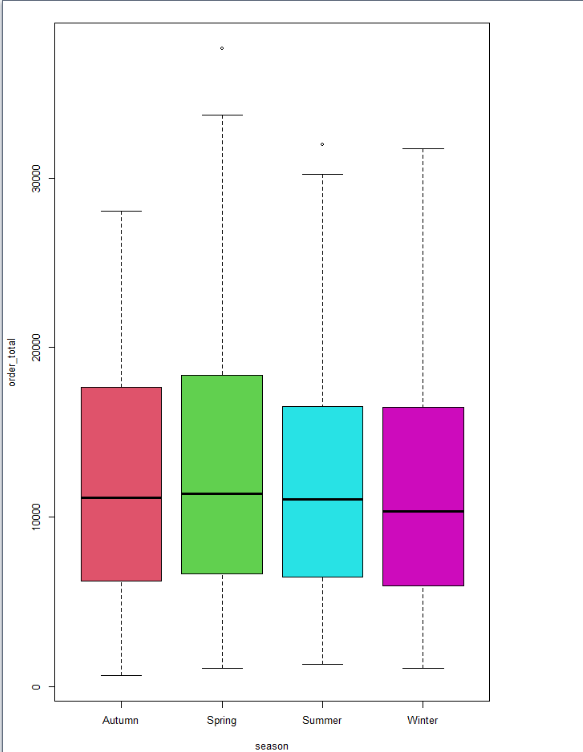
\includegraphics[scale =0.35]{IMAGES/12.png}
    \caption{Kết quả khi vẽ lại Boxplot thể hiện phân phối của order\_total theo season.}
    \label{fig21}
\end{figure}

\textbf{\textit{Nhận xét}}: Hình~\ref{fig21} Ta thấy boxplot tổng chi phí đặt hàng theo mùa cho thấy sự phân tán lớn giữa các mùa, với khoảng giữa (IQR) tương đối giống nhau. Mùa xuân có trung vị cao nhất, phản ánh chi phí đặt hàng thường cao hơn, trong khi mùa hè và mùa đông có trung vị thấp hơn. Một số giá trị ngoại lệ xuất hiện ở mùa xuân và mùa hè, cho thấy các đơn hàng có chi phí rất cao. Mặc dù phạm vi tổng chi phí các mùa tương tự, mùa xuân có xu hướng chi tiêu cao hơn, gợi ý mùa xuân là thời điểm mua sắm sôi động. Ta có thể dự đoán mùa không ảnh hưởng quá nhiều đến tổng chi phí đặt hàng.
\\
Ta tiến hành vẽ biểu đồ Boxplot thể hiện phân phối của order\_total theo nearest\_warehouse và tiến hành xử lí ngoại lai tương tự như biến season (\textbf{Code[102]$\rightarrow$[124]}).

\begin{figure}[H]
    \centering
    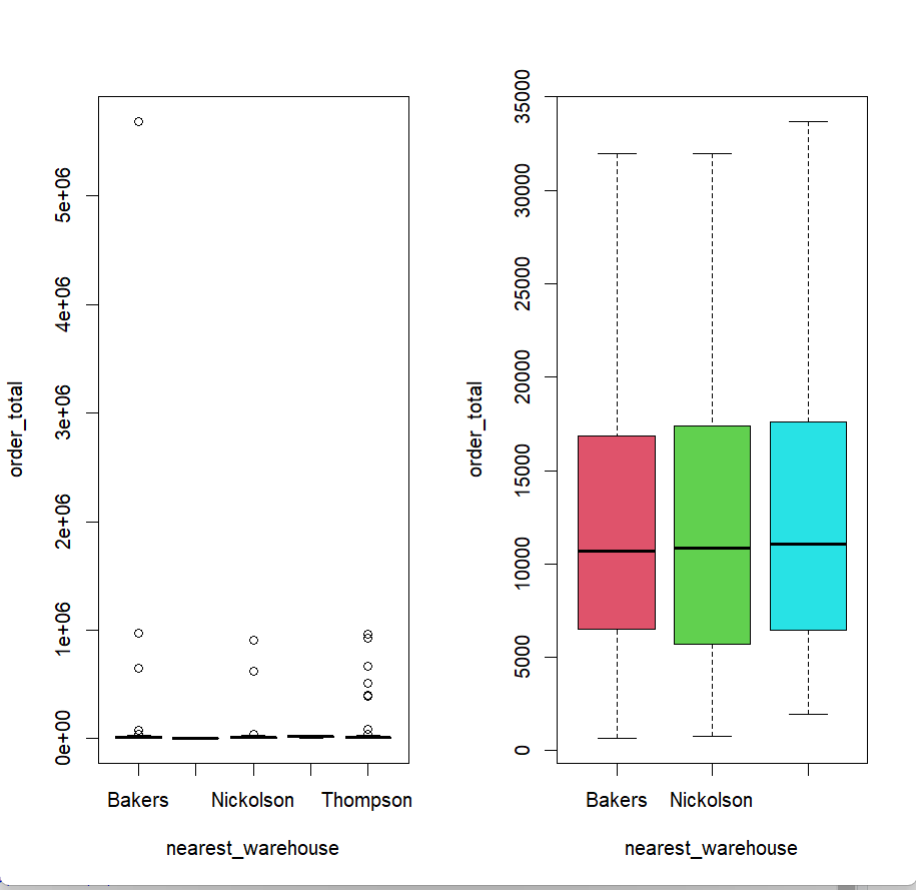
\includegraphics[scale=0.3]{
    IMAGES/18.png}
    \caption{Kết quả khi vẽ boxplot thể hiện phân phối của order\_total theo nearest\_warehouse.}
    \label{fig22}
\end{figure}
\textbf{\textit{Nhận xét}}: Hình~\ref{fig22} Ta thấy từ boxplot biểu diễn mối quan hệ giữa biến nearest\_warehouse (gồm các nhóm Bakers, Nickolson và Thompson) và biến order\_total cho thấy phân bố tổng đơn hàng của các nhóm khá tương đồng, với khoảng giá trị dao động từ 0 đến 35.000. Trung vị của order\_total ở ba nhóm gần nhau, không có sự chênh lệch rõ rệt về giá trị trung tâm. Phạm vi biến động của dữ liệu cũng tương đối giống nhau và không xuất hiện giá trị ngoại lệ đáng chú ý. 

Trong các nhóm, nhóm Thompson có tổng đơn hàng trung vị cao nhất, trong khi nhóm Bakers có trung vị thấp nhất, tuy nhiên sự khác biệt này không quá lớn. Nhìn chung, ta có thể kết luận rằng biến nearest\_warehouse không có ảnh hưởng đáng kể đến order\_total, và sự hài lòng của khách hàng ở các kho hàng này không tác động mạnh đến tổng số lượng đơn hàng.

Vẽ biểu đồ Boxplot thể hiện phân phối của order\_total theo is\_happy\_customer (\textbf{Code[130]}). Sau đó, ta thực hiện xử lí ngoại lai và vẽ lai đồ thị tương tự với hai biến trên (\textbf{Code[132]$\rightarrow$[149]}).
\begin{figure}[H]
    \centering
    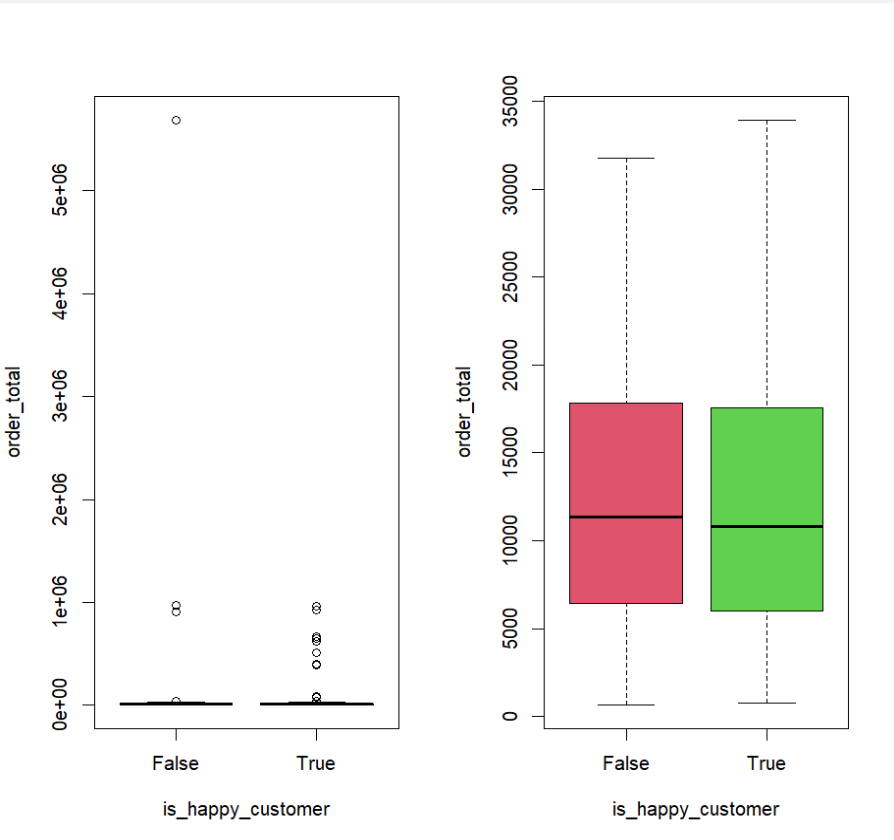
\includegraphics[scale=0.25]{IMAGES/19.png}
    \caption{Kết quả khi vẽ boxplot thể hiện phân phối của order\_total theo is\_happy\_customer.}
    \label{fig23}
\end{figure}
\textbf{\textit{Nhận xét}}: Hình~\ref{fig23} Ta thấy được đồ thị boxplot này biểu diễn mối quan hệ giữa biến is\_happy\_customer (gồm hai nhóm: False và True) và biến order\_total. Dưới đây là nhận xét:
\begin{itemize}
    \setlength{\itemsep}{-2pt}
  \item Ta thấy rằng các nhóm False và True có phân bố giá trị order\_total tương đối giống nhau, với khoảng giá trị từ 0 đến 35.000. Trung vị của nhóm True cao hơn nhóm False, cho thấy khách hàng hài lòng (True) có xu hướng chi tiêu cao hơn một chút, tuy nhiên sự khác biệt không lớn. Phạm vi giá trị và các chỉ số tứ phân vị cũng khá tương đồng giữa hai nhóm.


    \item Nhìn chung, ta có thể kết luận rằng biến is\_happy\_customer chỉ ảnh hưởng nhẹ đến order\_total, với mức chi tiêu trung bình của nhóm khách hàng hài lòng (True) nhỉnh hơn nhóm không hài lòng (False).
  \end{itemize}
Ta tiến hành vẽ biểu đồ Boxplot thể hiện phân phối của order\_total theo is\_expedited\_delivery và ta thực hiện xử lí ngoại lai và vẽ lại đồ thị tương tự (\textbf{Code[152$\rightarrow$[170]}).
\begin{figure}[H]
    \centering
    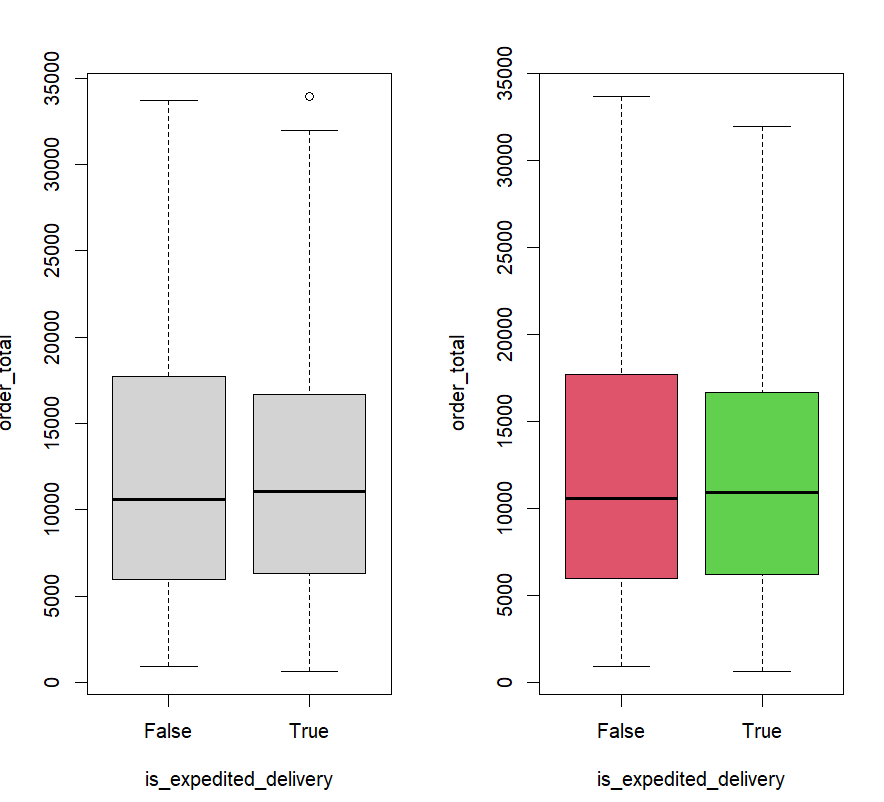
\includegraphics[scale=0.35]{
    IMAGES/20.png}
    \caption{Kết quả khi vẽ boxplot thể hiện phân phối của order\_total theo is\_expedited\_delivery.}
    \label{fig24}
\end{figure}
\textbf{\textit{Nhận xét}}: Hình~\ref{fig24} Dựa trên biểu đồ boxplot bên phải, ta thấy được biến is\_expedited\_delivery (việc giao hàng nhanh hay không) dường như không ảnh hưởng rõ ràng đến order\_total (tổng giá trị đơn hàng). Cụ thể: 

Ta nhận thấy rằng trung vị của hai nhóm (False và True) gần như bằng nhau, điều này cho thấy không có sự khác biệt lớn về giá trị trung bình giữa hai nhóm. Độ phân tán dữ liệu (thể hiện qua kích thước hộp và râu) của hai nhóm cũng tương đối giống nhau. Phân bố giá trị trong cả hai trường hợp là khá tương đồng, không có sự khác biệt rõ rệt.



\subsubsection{Đồ thị Scatter/Plot}
Ta thực hiện vẽ đồ thị Scatter/Plot theo biến order\_total và order\_price (\textbf{Code[175]}).
\begin{figure}[H]
    \centering
    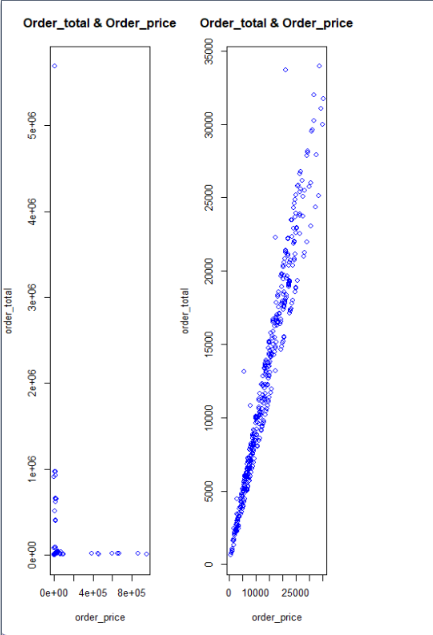
\includegraphics[scale=0.4]{
    IMAGES/21.png}
    \caption{Kết quả khi vẽ Scatter/plot thể hiện phân phối của order\_total và order\_price.}
    \label{fig25}
\end{figure}
\textbf{\textit{Nhận xét}}: Hình~\ref{fig25} Sau khi loại bỏ các điểm ngoại lai, ta thấy được đồ thị trở nên rõ ràng hơn và cho thấy một xu hướng tuyến tính giữa order\_price và order\_total. Cụ thể:
\begin{itemize}
\setlength{\itemsep}{0pt}
    \item Ta nhận thấy một quan hệ tuyến tính rõ ràng giữa hai biến. Biểu đồ cho thấy sự tăng trưởng gần như tuyến tính: khi giá trị của order\_price tăng lên, order\_total cũng tăng theo, thể hiện qua việc các điểm dữ liệu xếp thành một đường chéo tăng dần.
    \item Ta cũng nhận thấy một mối quan hệ tương quan dương mạnh, với hầu như không có dữ liệu bị phân tán hoặc nằm ngoài xu hướng chính, chứng tỏ rằng hai biến có mối quan hệ tỷ lệ thuận.
    \item Kết quả này gợi ý rằng sự gia tăng của giá trị đơn hàng (order\_price) sẽ dẫn đến sự gia tăng tương ứng của tổng đơn hàng (order\_total), điều này có thể do tính chất cộng gộp của dữ liệu. Mối quan hệ này phù hợp với các hệ thống thương mại, nơi tổng số tiền phụ thuộc vào giá trị từng đơn hàng.
\end{itemize}
Ta  vẽ đồ thị Scatter/plot cho order\_total và distance\_to\_nearest\_warehouse (\textbf{Code[177]}).
\begin{figure}[H]
    \centering
    \captionsetup{justification=centering, margin = 2cm}
    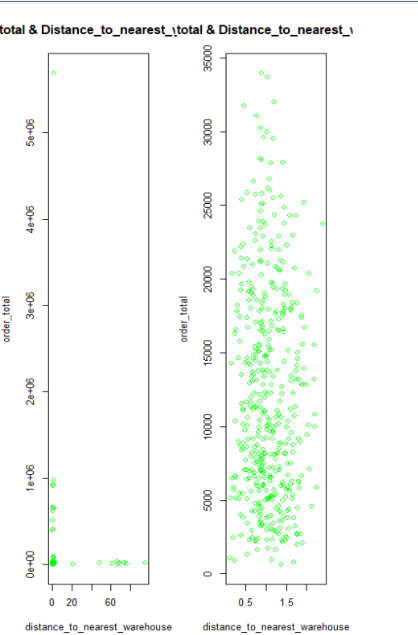
\includegraphics[scale =0.3]{IMAGES/22.png}
    \caption{Kết quả khi vẽ Scatter/plot thể hiện phân phối của order\_total và distance\_to\_nearest\_warehouse.}
    \label{fig26}
\end{figure}
\textbf{\textit{Nhận xét}}: Hình~\ref{fig26} Như vậy, ta vẫn chưa thấy được giữa hai biến distance\_to\_nearest\_warehouse và order\_ total có quan hệ tuyến tính. Ta có thể dự đoán biến distance\_to\_nearest\_warehouse không ảnh hưởng đến biến order\_total.
\\
Ta tiếp tục vẽ đồ thị Scatter/plot cho order\_total và delivery\_charges (\textbf{Code[176]}).
\begin{figure}[H]
    \centering
    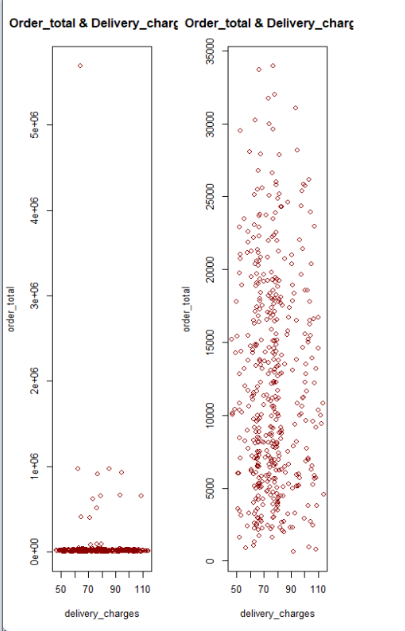
\includegraphics[scale=0.3]{
    IMAGES/23.png}
    \caption{Kết quả khi vẽ Scatter/plot thể hiện phân phối của order\_total và delivery\_charges.}
    \label{fig27}
\end{figure}
\textbf{\textit{Nhận xét}}: Hình~\ref{fig27}
Sau khi ta xóa điểm ngoại lai, ta vẫn chưa thấy được sự quan hệ tuyến tính rõ ràng giữa hai biến delivery\_charges và order\_total. Ta có thể dự đoán rằng biến delivery\_charges không ảnh hưởng đến biến order\_total.
\\
Ta tiếp tục vẽ cho order\_total và coupon\_discount (\textbf{Code[178]}). 
\begin{figure}[H]
    \centering
    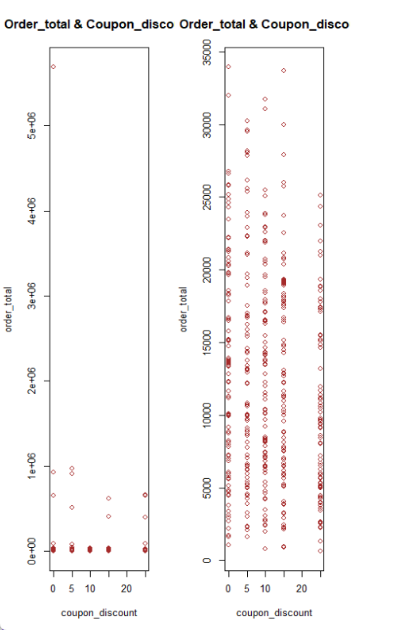
\includegraphics[scale=0.4]{
    IMAGES/24.png}
    \caption{Kết quả khi vẽ Scatter/plot thể hiện phân phối của order\_total và coupon\_discount.}
    \label{fig28}
\end{figure}
\textbf{\textit{Nhận xét}}: Hình~\ref{fig28} Dựa trên biểu đồ scatter plot, ta thấy được mối quan hệ giữa coupon\_discount (giảm giá phiếu giảm giá) và order\_total (tổng đơn hàng) không rõ ràng. Giá trị coupon\_discount chủ yếu tập trung ở mức thấp (dưới 10), trong khi order\_total có sự phân tán rộng, dao động từ thấp đến hơn 30,000. Dữ liệu cho ta thấy hai biến không có xu hướng tuyến tính hoặc phi tuyến rõ rệt, cho thấy mức giảm giá không có ảnh hưởng trực tiếp hoặc có nhưng rất ít đến tổng chi phí đơn hàng.



